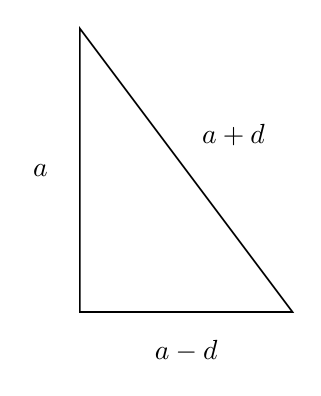
\begin{tikzpicture}[x=1cm,y=1cm,font=\normalsize,
 geometry edge/.style={solid,line width=.6pt},
 geometry mark/.style={solid,line width=.6pt},
 geometry label/.style={font=\normalsize,inner sep=2pt}]
\coordinate (V1) at (0,0);
\coordinate (V2) at (0,3.6);
\coordinate (V3) at (2.7,0);
\coordinate (Sa) at (-0.5,1.8);
\coordinate (Sb) at (1.35,-0.5);
\coordinate (Sc) at (1.95,2.25);
\draw[geometry edge] (V1)--(V2)--(V3)--cycle;
\node[geometry label] at (Sa) {$a$};
\node[geometry label] at (Sb) {$a-d$};
\node[geometry label] at (Sc) {$a+d$};
\end{tikzpicture}
